%-------------------------------------------------------------------------------------------
% Vorlage erstellt von sli92
% Latex für Einsteiger: http://latex.mschroeder.net/#textformatierung
% Formeln in Latex: http://www.hosi.de/latex/mathe.htm
%-------------------------------------------------------------------------------------------
%PRÄAMBEL
%-------------------------------------------------------------------------------------------

\documentclass[a4paper,14pt,headsepline]{scrartcl}

\usepackage[ngerman]{babel}
\usepackage[utf8]{inputenc}
\usepackage{fancyheadings}
\usepackage{graphicx}
\usepackage{eurosym}

\usepackage{hyperref}

% Absatzeinrückung
%++++++++++++++++++++++++++
%\setlength{\parskip}{5pt}
%\setlength{\parindent}{0pt}

\setlength{\parskip}{1.5em}
\setlength{\parindent}{0pt}

% Kopf- und Fußzeile
%++++++++++++++++++++++++++

\pagestyle{fancy}
\lhead{\bfseries netcon}
%\chead{Lipp}
\rhead{\nouppercase{\leftmark}}

%C für Center
\fancyfoot[C]{ \thepage}

%-------------------------------------------------------------------------------------------
%DOKUMENT
%-------------------------------------------------------------------------------------------

\begin{document}

% Titelseite
%++++++++++++++++++++++++++
\author{Lipp, Pietryka} 
\title{Diplomarbeit: netcon} 
\date{} 
\maketitle

\newpage

\section*{Zusammenfassung}
\newpage

\section*{Abstract}
\newpage

\section*{Danksagung}
\newpage

\section*{Vorwort}
Sie wollen Umweltgrößen an mehreren Standorten (aus der Ferne) überwachen? An den Standorten ist lediglich ein gemeinsames Ethernet-Netzwerk verfügbar und für den Aufbau eines eigenen Netzes fehlt das Budget?

Im Rahmen dieser Diplomarbeit, wurde mit \textbf{netcon} ein quelloffenes, flexibles Messsystem auf Ethernet-Basis geschaffen.\footnote{Maßnahmen für die spätere Implementierung eines Aktornetzwerks wurden getroffen. Diese wurde aber aus Zeitgründen nicht durchgeführt. } Dabei wurde darauf Rücksicht genommen, erfahrene Endanwender, Unternehmen und Entwickler gleichermaßen zu bedienen. Je nach Anwendungsfall und Vorkenntnissen sollten Sie in der Lage sein ihr eigenes Messsystem aufzubauen. 

Im ersten Kapitel folgt ein Überblick über die \textbf{allgemeine Konzeption} - Systemvoraussetzungen, Aufbau, Schnittstellen und grundsätzliche Funktionsweise. Ein zweites Kapitel gibt eine Einführung in \textbf{grundlegende Begriffe}, die für ein tieferes Verständnis der Entwicklungen erforderlich sind. Danach folgt das große Kapitel, \textbf{Hardware}, das den Aufbau und die Funktionsweise der Messmodule behandelt, sowie in die genaue Verwendung der Schnittstellen und Protokolle auf der Hardwareseite einführt. Das letzte Kapitel, \textbf{Software} beschreibt die Verwaltungsschicht und dessen Interfaces für die Anzeige der Moduldaten.  

\newpage

% Inhaltsverzeichnis
%++++++++++++++++++++++++++
\tableofcontents
\newpage

%Inhalt
%++++++++++++++++++++++++++

\section{Überblick [Lipp]}

Netcon ist zum einen ein Messsystem zur Einbindung in ein bestehendes Ethernet-Netzwerk, zum anderen aber auch das Ziel flexible Werkzeuge für die Erstellung eines solchen Systems bereitzustellen. Dabei stehen alle Entwicklungen unter OpenSource. 

Da das System als Übertragungsmedium die Ethernet-Schnittstelle mit der TCP/IP-Protokollschicht verwendet, ist Echtzeitverhalten nicht garantiert. Dadurch ist es nur für unzeitkritische Aufgaben geeignet. 

\subsection{Zielgruppen}
Erfahrene Endandwender, genauso Entwickler sollten mit netcon in der Lage sein, ein Messsystem zu realisieren. Es wurden hardware- und softwareseitig einfache Schnittstellen geschaffen um je nach Wunsch und vorherrschenden Kenntnissen eigene Anwendungen zu erstellen. 

Der Anwender kann sich entscheiden, entweder entwickelt er auf Basis der Spezifikationen die netzwerkfähigen Module selbst, oder aber er verwendet die im Rahmen dieser Diplomarbeit gewählten Mikrocontroller-Systeme. Dazu stellt netcon die entwickelte Firmware zur Verfügung. Weiters besteht für netzwerktechnisch unerfahrene Entwickler die Möglichkeit, ihre Module netzwerkfähig zu machen.

Auch auf der Softwareseite stehen mehrere Wege offen. Entwickler können eigene Applikationen über die Schnittstelle der Verwaltungsschicht aufsetzen, oder aber auch die entwickelte Weboberfläche zur Anzeige und Steuerung der Module verwenden.

\subsection{Anwendungsbeispiele}
Netcon sieht in seiner Spezifikation mehrere Typen von Messmodulen vor. Folgende Liste zeigt Anwendungen, die unter anderem mit diesem System verwirklicht werden können:
\begin{itemize}
	\item Spannungsmessung
	\item Temperaturmessung
	\item Zeitmessung
\end{itemize}

\newpage

\subsection{Systemvoraussetzungen}

Das netcon Messsystem wurde für dein Einsatz in einem Ethernet-Netzwerk konzipiert. Dieses muss zumindest über folgende Komponenten verfügen:
\begin{itemize}
	\item Anschlussmöglichkeiten für die Module (Router/Switch/WLAN)
	\item DHCP-Server für die IP-Adressvergabe
	\item \textbf{Server} - Javafähige Betriebsumgebung für die Verwaltungsschnittstelle z.B. PC, Embedded System
	\item \textbf{Client} - Anzeigegerät z.B. Smartphone, Computer
\end{itemize}

Zusätzlich wird gegebenenfalls ein PHP-fähiger Webserver benötigt, um die bereits entwickelte Website verwenden zu können. Die genauen Anforderungen an die Softwareumgebung, sowie die Einrichtung einer Java Runtimte Environment (JRE) und eines Webservers sind im Kapitel Software nachzulesen.

Und nicht zu vergessen sind die wichtigsten Komponenten, die netzwerkfähigen Module. Diese können, wie bereits erwähnt, nach den netcon-Protokollen selbst entwickelt, oder aber auch nach Anleitung erstellt werden. Dazu mehr im nächsten Abschnitt.
\newpage

\subsection{Systemaufbau}
Im folgenden sind die zwei grundlegenden netcon-Komponenten inkl. ihrer Schnittstellen beschrieben. Je nachdem wie netcon genutzt werden soll, wird auf weitere Kapitel verwiesen.

\subsubsection{Module}
Die \textbf{Module} sind Hardware, die über Ethernet und TCP/IP erreichbar und abfragbar sind. 

\begin{figure}[h]
\begin{center}
\fbox{
	%Rahmengroesse	
	\begin{minipage}{0.7 \paperwidth}
	\begin{center}
	%Bildgroesse
	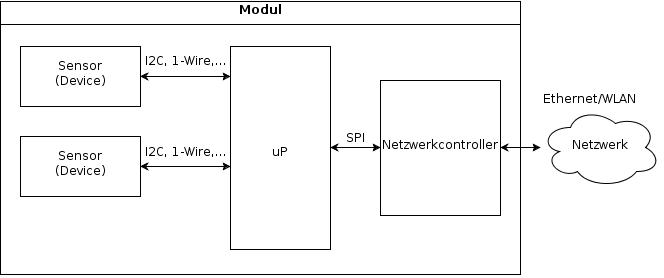
\includegraphics[width=0.5 \paperwidth]{./bilder/modul_aufbau.png}
	\caption{Aufbau eines Moduls}
	\label{modulaufbau}
	\end{center}
	\end{minipage}
}
\end{center}
\end{figure}

\newpage

Sie vereinen alle benötigten Komponenten - Mess- und Netzwerkeinheit - auf einer Platine (siehe Abb. \ref{modulaufbau}). Hier erfolgt die Übertragung zwischen den Sensoren und dem Mikroprozessor (uP) meist über Schnittstellen, wie I2C oder 1-Wire, während der Netzwerkcontroller per SPI mit dem uP kommuniziert. Über TCP und mit den beiden Protokollen \textit{netfind} und \textit{netcon} erfolgt die Abfrage und Steuerung durch den plattformunabhängigen Verwaltungs-Deamon \textit{netcond}. Näheres dazu im nächsten Abschnitt. 

\textbf{Messmodule} umfassen beispielsweise Sensoren für Temperatur, Luftdruck und Zeit. Jeder dieser Sensoren wird von netcon als \textbf{Device} bezeichnet und kann mit seiner ID abgefragt werden.

Um den Modulen automatisch eine IP-Adresse zuweisen zu können und damit Konfigurationsarbeit zu ersparen, sollten diese auch das DHCP-Protokoll unterstützen.

Es bestehen grundsätzlich drei Möglichkeiten zur Erstellung von Modulen. Wenn Sie alle erforderlichen Kenntnisse besitzen, um die gesamte Entwicklung selbst zu übernehmen, informieren Sie sich im Kapitel Hardware über den Aufbau der netcon-Protokolle. Sind Sie in der Lage einfache Messmodule ohne Netzwerkfähigkeit zu erstellen, verbinden Sie doch ein zusätzliches Netzwerkmodul (siehe Abb. \ref{modulaufbau2}). Diese Möglichkeit erfordert lediglich die Implementierung der Seriellen Schnittstelle (UART). Genauso können die im Rahmen dieser Diplomarbeit konzpierten Module mit ihrer Firmware für die Erstellung eigener Module herangezogen werden. Egal welche Wahl Sie treffen, das Kapitel Hardware unterstützt Sie in allen drei Fällen.

\begin{figure}[h]
\begin{center}
\fbox{
	%Rahmengroesse	
	\begin{minipage}{0.8 \paperwidth}
	\begin{center}
	%Bildgroesse
	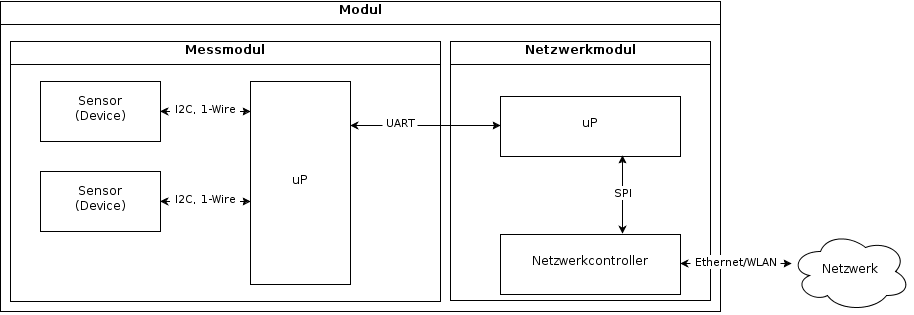
\includegraphics[width=0.7 \paperwidth]{./bilder/modul_aufbau2.png}
	\caption{Netzwerkfähiges Messmodul mittels LAN-UART Umsetzer}
	\label{modulaufbau2}
	\end{center}
	\end{minipage}
}
\end{center}
\end{figure}

\newpage

\subsubsection{Software}
Die Verwaltungsschnittstelle \textbf{netcond} ist eine in Java geschriebene Hintergrundanwendung (Daemon), die sich um die Verwaltung der Module kümmert. Wie in Abb. \ref{netcond} erkennbar können über das netcon Application Interface (netcon API) per TCP die Moduldaten abgefragt werden. Die Anwendung kann beispielsweise eine Website auf einem Webserver oder ein Smartphone-App sein. 

\begin{figure}[h]
\begin{center}
\fbox{
	%Rahmengroesse	
	\begin{minipage}{0.7 \paperwidth}
	\begin{center}
	%Bildgroesse
	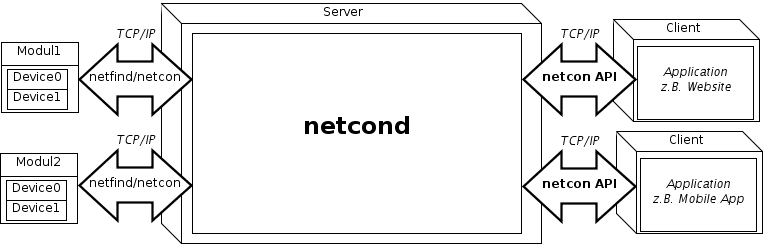
\includegraphics[width=0.7 \paperwidth]{./bilder/netcond.png}
	\caption{netcond}
	\label{netcond}
	\end{center}
	\end{minipage}
}
\end{center}
\end{figure}

\newpage
Soll die Anwendung zur Anzeige der Messdaten selbst entwickelt werden, führt das Kapitel Software in die Verwendung der Softwareschnittstelle ein. Sonst kann die bereits entwickelte Website \textbf{netcon web} (siehe Abb. \ref{website}) verwendet werden. Dazu ist zusätzlich zur JRE ein http-Webserver mit PHP-Unterstützung erforderlich. Deren Installation und Konfiguration ist im Kapitel Software erklärt. 

\begin{figure}[h]
\begin{center}
\fbox{
	%Rahmengroesse	
	\begin{minipage}{0.7 \paperwidth}
	\begin{center}
	%Bildgroesse
	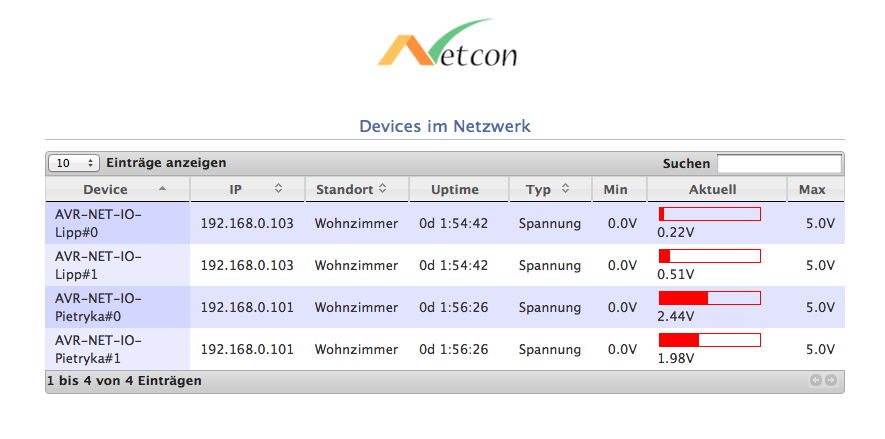
\includegraphics[width=0.7 \paperwidth]{./bilder/website.png}
	\caption{netcon web}
	\label{website}
	\end{center}
	\end{minipage}
}
\end{center}
\end{figure}

\newpage

\subsection{Funktionsweise}

\begin{figure}[h]
\begin{center}
\fbox{
	%Rahmengroesse	
	\begin{minipage}{0.8 \paperwidth}
	\begin{center}
	%Bildgroesse
	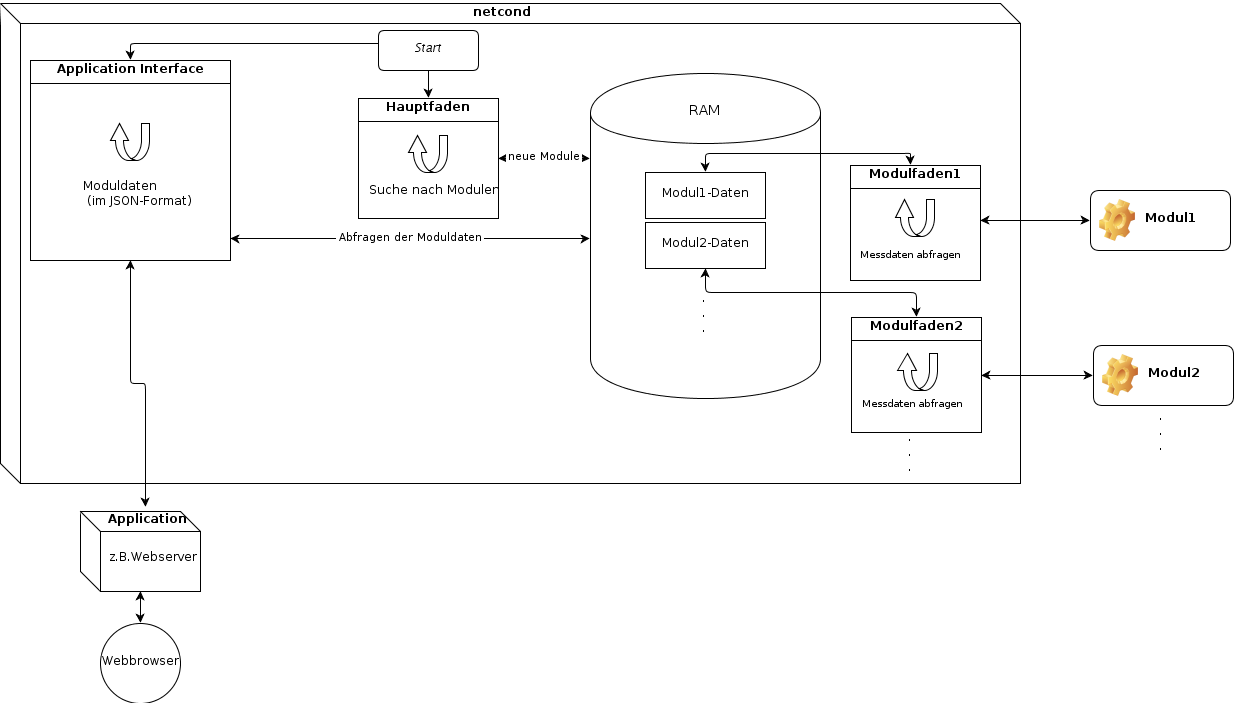
\includegraphics[width=0.8 \paperwidth]{./bilder/funktionsweise.png}
	\caption{netcon - Funktionsprinzip}
	\label{funktionsweise}
	\end{center}
	\end{minipage}
}
\end{center}
\end{figure}

Der Java-Daemon netcond sucht nach dem Start alle paar Sekunden das Netzwerk nach verbunden Modulen ab und halt diese in einer Liste. Für jedes dieser Module wird ein neuer Programmfaden erzeugt, der ständig Messdaten abfragt und diese speichert. Zusätzlich startet der Daemon einen weiteren Subprozess, die Schnittstelle, über die eine Anwendung - in diesem Fall ein Webserver - die Daten abfragen kann. Verbindet sich ein Webbrowser zu diesem Webserver, weißt ein PHP-Script den Daemon an, die aktuellen Daten zu übermitteln. Diese werden dann auf der Website angezeigt. Dieses Prinzip ist nocheinmal in Abb. \ref{funktionsweise} grafisch verdeutlicht.

\newpage


\section{Grundlagen [Pietryka]}
\subsection{OSI-Schichtenmodell}
Das OSI-Schichtenmodell ist ein von der ISO im Jahre 1983 standardisiertes Modell, welches als Designgrundlage für Kommunikationsprotokolle in Computernetzen dient. Dabei wird die Kommunikation beim OSI-Modell auf sieben Schichten bzw. Layern aufgeteil. Für jede dieser Schichten sind Anforderungen und Aufgaben definiert, welche von entsprechenden Protokollen realisiert werden müssen. Eine konkrete Umsetzung ist aber nicht vorgegeben, daher gibt es für eine Schicht mehrere in Frage kommenden Protokolle.
\subsubsection{Schicht 1: Physical Layer}

 
\subsection{Ethernet}
\subsection{IP}
\newpage

\section{Hardware [Pietryka]}
\subsection{Auswahl des Ethernet Controllers}
Damit ein Mikrocontroller über das Ethernet kommunizieren kann, wird eine entsprechende Hardware benötigt, der sogenannte Ethernet Controller. Ein Ethernet Controller übernimmt dabei die Aufgaben der OSI-Schichten 1(Physical) und 2(Data-Link). Der Controller benötigt zudem einen entsprechend großen Empfangspuffer, um mindestens einen vollwertigen Ethernet-Frame(1542 Byte) aufzunehmen zu können. Dabei standen für 8-Bit Mikrocontroller vorerst zwei verschiedene Bausteine zur Auswahl, einmal der CP2200 von SiLabs, und einmal der ENC28J60 von Microchip. Beide Controller haben, was die Netzwerkkommunikation angeht, so ziemlich die selben Features, der gravierende Unterschied liegt jedoch in der Ansteuerung dieser. Der CP2200 wurde von SiLabs, wie es scheint, nur für die Verwendung mit einem Mikrocontroller vom Typ 8051 entwickelt, die Ansteuerung erfolgt deshalb über einen parallelen Adress-/Datenbus wodurch man mindestens 16 Leitungen und Pins am Mikrocontroller benötigt. Beim ENC28J60 erfolgt die Kommunikation über den SPI-Bus, daher benötigt man nur vier Leitungen(MOSI, MISO, SCK, CS), dadurch hat auch der Netzwerkcontroller selber nur 28 Pins und ist auch im "bastlerfreundlichen" DIP-Gehäuse zu bekommen. Ein anderer Faktor für die Auswahl des ENC28J60 war das Vorhandensein einer günstigen Entwicklungsplatine, es gibt bei Pollin den AVR-NET-IO Bausatz, dieser kostet nur \EUR{20} und enthält alle für die Netzwerkprogrammierung benötigten Komponenten(ATmega32, ENC28J60, RJ-45 Buchse).

\subsection{ENC28J60 Beschaltung}
Die Aussenbeschaltung benötigt neben einigen Standardbauelementen auch einige 1\% Widerstände und einen 1:1 Übertrager, jedoch gib es RJ-45 Buchsen in denen bereits der Übertrager, sowie die LEDs bereits eingebaut sind.
\begin{figure}[h]
\begin{center}
\fbox{
	%Rahmengroesse	
	\begin{minipage}{0.7 \paperwidth}
	\begin{center}
	%Bildgroesse
	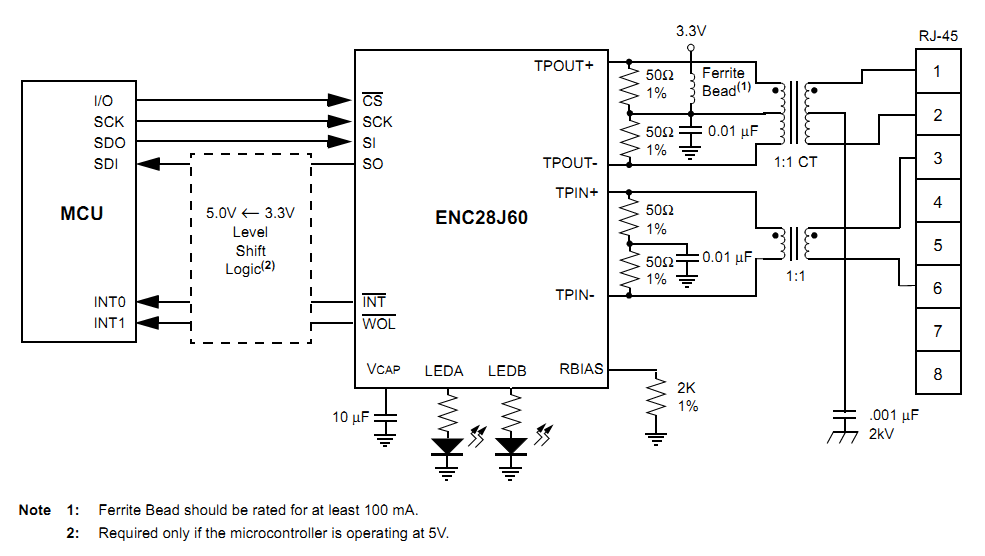
\includegraphics[width=0.7 \paperwidth]{./bilder/enc28j60_beschaltung.png}
	\caption{Aussenbeschaltung ENC28J60}
	\end{center}
	\end{minipage}
}
\end{center}
\end{figure}



\subsection{ENC28J60 Treibersoftware}

\newpage
\section{Software [Lipp]}

\subsection{Aufgaben}
was sind die grundsätzlichen aufgaben der Software, wofür ist sie da?

\subsection{Java}
warum java?

\subsection{Aufbau und Funktionsweise}
Aufbau der Software
Programmabläufe (Flussdiagramme)
Genaue Beschreibung der Schnittstellen

\subsection{Installation}

\subsubsection{JRE}

\subsubsection{Webserver}

 
\end{document}